\chapter{Work Done}

\section{Java Implementaion}

I have implemented a simple tic-tac-toe game in Java that utilizes alpha-beta pruning so that the computer can play against computer users. The structure of the game is as following:

\begin{itemize}
	\itemsep-0.5em 
	\item TicTacToe, the driver class for the game.
	\item GameFrame, the graphical user interface class.
	\item GameController, the logic implementaion class.
\end{itemize}

I have added the ability to change the level of difficulty of the game, so there are {\bf Easy}, {\bf Medium} and {\bf Hard} levels.

\section{Game Testing}

\begin{center}
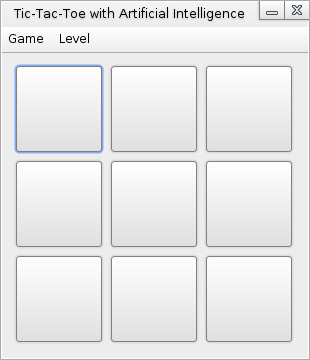
\includegraphics[width=0.45\textwidth]{./game1}
\hspace*{0.1em}
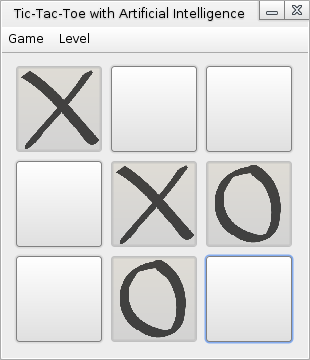
\includegraphics[width=0.45\textwidth]{./game2}

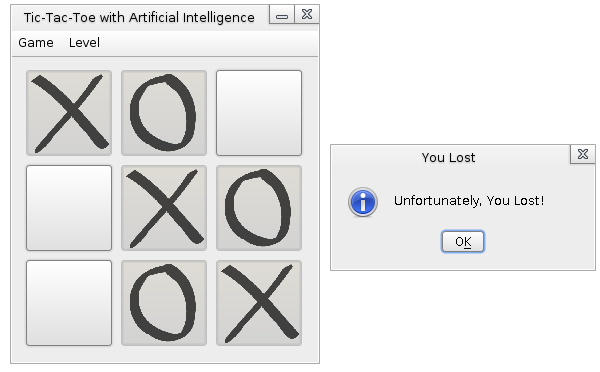
\includegraphics[width=0.9\textwidth]{./game3}
\vspace*{0.3em}

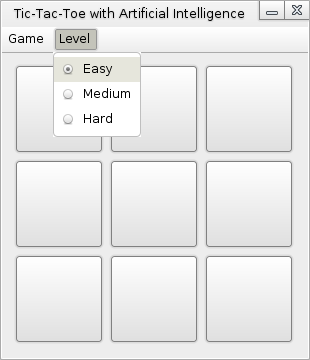
\includegraphics[width=0.45\textwidth]{./game4}
\hspace*{0.1em}
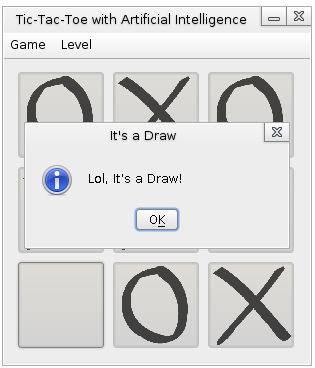
\includegraphics[width=0.45\textwidth]{./game5}

\end{center}